\section{Introduction}
So far we have seen \textbf{Supervised Learning} which goal is, given data $(\textbf{X},y)$, to learn a function that maps $f: \textbf{X} \longrightarrow y$. For example, regression or image captioning belong to this machine learning tasks category. 

Another fundamental class of tasks is \textbf{Unsupervised learning} which, given only data \textbf{X}, the algorithm learns some underlying hidden structure. For example, clustering and densisty estimation taks belong to such class.

In general, models that belong to unsupervised learning can  be splitted into 2 categories: \textbf{non probabilistic} and \textbf{probabilistic generative}. The latter will be the scope of this chapter.

\section{Generative Models}
The goal of this class of models is to solve the so called \textbf{density estimation} task. 


Given a training data with a certain $\text{training data distribution }  \sim p_{data}(x)$, the model aims to approximate this underlying distribution in order to be able to generate new samples. To do that, the model learns a $\text{Generated samples distribution } \sim p_{model}(x)$, such that $ p_{model}(x)$ is as similar as possible to $ p_{data}(x)$.


We can further categorize generative models based on whether or not the sample density has been explicitly specified, namely \textbf{Explicit Density Estimation models} (e.g. $p_{model}(x)$ should be a normal distribution whose parameters are unknown), and \textbf{Implicit Density Estimation} models. The latter differs because the model can sample from $p_{model}(x)$ without explicitly defining the density function.

One reason to use generative models is to simulation purposes (e.g. reinforcement learning, transform synthetic data into realistic ones).

\section{Implicit Density Estimation}

\subsection{Generative adversarial networks (GAN)}

GANs are generative probabilistic models that do not consider any explicit density function, rather they just focus on training with an adversarial approch a model to generate sample from a simple distribution to a complex one similar to training data. GANs address this task by implementing the interplay of the two "players" (networks), namely the Discriminator and Generator.

The idea is to first sample from a simple distribution (e.g. random noise) and learn a transformation function, i.e. a neural network called \textbf{Generator}, that reproduces and generates samples from training distribution. Hence, the Generator should be able to produce samples as similar as possible to training data in order to fool a second neural network, called \textbf{discriminator}, which aims to discriminate between real and generated ("fake") samples. The two parties are \textbf{adversarial}, meaning that they share the \textbf{same loss}.  This choice affects training stability. 


\begin{figure}[!htbp]
    \centering
    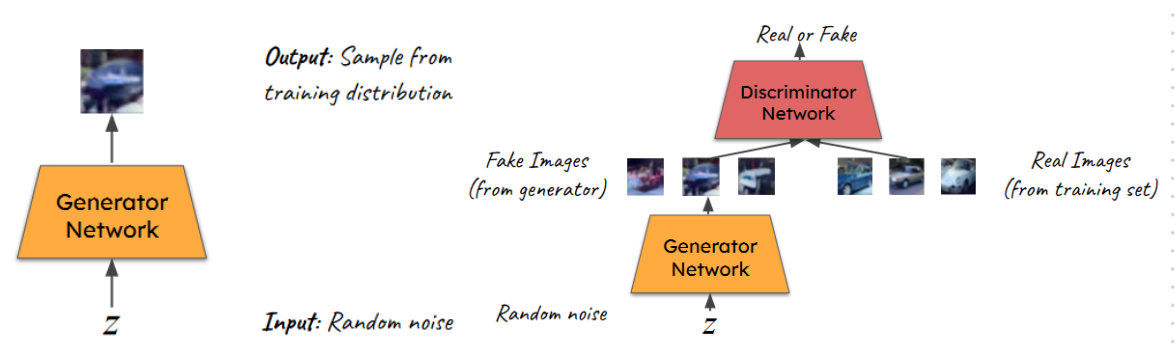
\includegraphics[width=\linewidth]{tikz/GAN.png}
    \caption{{\color{red}\colorbox{pink}{Tikz TO-DO}} \textbf{Left}: the figure shows a global view of the Generator model. $z$ represents a simple distribution from which sample from and feed a NN to transform the simple distribution to the target (similar and complex) one; \textbf{Right}: the figure shows a global view of the GAN model whit its two parties. The Discriminator NN classifier is needed in order to discriminates samples.}
    \label{fig:GAN}
\end{figure}

Depending on what we use for both \textbf{Generator} and \textbf{Discriminator} module, we will obtain different results also in terms of image quality. 

\paragraph{Loss}

The training procedure involves training jointly the two "players" and finds the distribution parameters by a min-max optimization problem: 

\begin{equation}\label{eq: GAN-loss}
    min_{\theta_{g}} max_{\theta_{d}}\left[E_{x \sim p_{data}}log D_{\textcolor{green}{\theta_{d}}(x)} + E_{z \sim p_{z}}log (1-D_{\textcolor{green}{\theta_{d}}}(G_{\textcolor{red}{\theta_{g}}(z))})  \right]
    \caption{{\color{red}\colorbox{pink}{Tikz TO-DO}} The equation shows the loss function of GAN model. The \textcolor{green}{green} part defines the disciminator output for real data (x); The \textcolor{red}{red} part defines the discriminator output for generated fake data ($G(z)$)}
\end{equation}

 Each of the two networks has its own parameter, namely \textcolor{green}{$\theta_{d}$} for the Discriminator, and  \textcolor{red}{$\theta_{g}$} for the Generator. Each of the two modules are described by a function, namely $D_{\theta_{d}}(x)$ and $G_{\theta_{g}}(z)$.

The loss is basically a \textbf{cross-entropy loss}: 
the Discriminator is a classifier, meaning that the final output will be a label real/fake. In order to produce it,  the Discriminator computes likelihoods for both real/fake data. The probability for real data comes from $log D_{\theta_{d}}(x)$, whereas for fake data  $log(1-D_{\theta_{d}}(G_{\theta_{g}}(z))$ . The \textbf{expectation terms} refers to the distribution where each sample is sampled from: $E_{x \sim p_{data}}$ samples from the training data, $E_{z \sim p_{z}}$ samples data from the simple distribution, which later is processed by the Generator $G_{\theta_{g}}(z)$ to process a synthetic fake image which is evaluated through the Discriminator $D_{\theta_{d}}$  to produce the likelihood.

\paragraph{Training}

As we have an adversarial architecture, during training we solve a \textbf{min-max} problem where each term represents the goal that each player try to pursue.


For the Discriminator, we want to find the set of parameters 
\textcolor{green}{$\theta_{d}$} that maximizes the objective function (equation \ref{eq: GAN-loss}) such that the likelihood for the Discriminator to discriminate between real and fake images is close to 1 (it is successful at its job); \textbf{At the same time}, for the Generator, we want find the set of parameters 
\textcolor{green}{$\theta_{g}$} that minimize the objective function such that the likelihood for the Discriminator to correctly discriminate between real and fake images is close to 0, thus the Generator is successful at fooling the opponent.


We use SGD alternating between \textbf{gradient ascent} on the discriminator and \textbf{Gradient descent} on the Generator, respectivelly :

\begin{equation}
\begin{aligned}
    &\max_{\theta_{d}} \left[E_{x \sim p_{data}} \log D_{\theta_{d}}(x) + E_{z \sim p_{z}} \log (1 - D_{\theta_{d}}(G_{\theta_{g}}(z))) \right] \\
    &\min_{\theta_{g}} \left[E_{z \sim p_{z}} \log (1 - D_{\theta_{d}}(G_{\theta_{g}}(z))) \right]
\end{aligned}
\end{equation}


The function to be optimized is complex, thus the training is \textbf{unstable}. Furthermore, it is very hard to monitor the process of the GAN because the objective function is not correlated to the quality of generated samples.


\begin{figure}[!htbp]
    \centering
    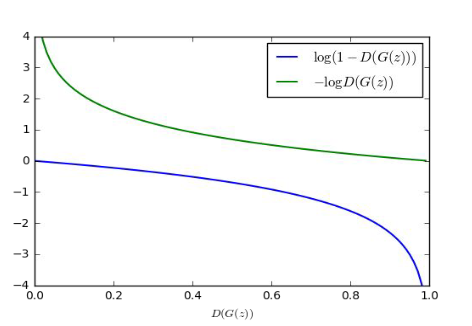
\includegraphics[width=\linewidth]{tikz/SGD GAN.png}
    \caption{{\color{red}\colorbox{pink}{Tikz TO-DO}} SGD for Generator in GAN}
    \label{fig:SGD-GAN}
\end{figure}




Figure \ref{fig:SGD-GAN} shows the gradient descent for
$log (1-D_{\theta_{d}}(G_{\theta_{g}}(z)))$(\textcolor{blue}{blue line}): the left part represents the gradient  when generated sample is likely fake. In this area, the gradient is very \textbf{flat} and corresponds to the region  where the model should be learning more to improve its generation capacity.  Conceptually, \textbf{we waste a lot of resources in our area of interest, making the learning more difficult}. Conversely, in the right part the gradient signal dominates, meaning that the sample is already good  and it is not useful for learning purposes. Thus, a way to improve the training is to modify this part of the objective function and transform it into a \textcolor{green}{ maximization problem}:

$$max_{\theta_{g}} E_{z\sim p(z)}log (D_{\theta_{d}}(G_{\theta_{g}}(z))) $$

This means that, instead of minimizing the likelihood of discriminantor being correct, the model now maximizes the likelihood of discriminator \textbf{being wrong}. As shown by the \textcolor{green}{green curve}, now the flat area has been inverted in the region out of our interest. 

Hence, the new training procedure requires to alternate between two \textbf{gradient ascent} procedures:

\begin{equation}
\begin{aligned}
    &\max_{\theta_{d}} \left[E_{x \sim p_{data}} \log D_{\theta_{d}}(x) + E_{z \sim p_{z}} \log (1 - D_{\theta_{d}}(G_{\theta_{g}}(z))) \right] \\
    &\max_{\theta_{g}} \left[E_{z \sim p_{z}} \log (D_{\theta_{d}}(G_{\theta_{g}}(z))) \right]
\end{aligned}
\end{equation}

Although the training efficiency has been improved, still there are some stability issues.

\paragraph{Inference}

In probabilistic generative models, the inference phase is called \textbf{sampling phase}: after the training, the Discriminator  is discarded and the Generator is used to produce samples similar to the training data from random noise.

Conceptually, the \textbf{Discriminator is just an auxiliary object} to match the distribution learnt by the Generator to the distribution of our data.



Results showed that if this version of GAN is trained in an unconstrained dataset, i.e. labels' distribution is very broad (MNIST is an easy dataset as digit have similar distribution, whereas CIFAR-10 is a more complex one), it performs poorly independently on which models are plugged to both Generator and Discriminator (like FC networks or CNN). However, advantages of using the Generator network are that it can be used as CNN backbone or NPL.

In the following sections we will analyse the main problems of GANs and see some papers that tried to mitigate them. Those problems can be listed as follows:

\begin{enumerate}
    \item We do not know if the model is overfitting and how to control it properly
    \item We do not know how to evaluate a GAN
    \item Training stability 
    \item Parameters can oscillate or diverge, Generator loss does not correlate with sample quality
\end{enumerate}



\subsection{DCGAN}




DCGAN represents the first deep convolutional architectures for GANs and was the first model for large resolution image generation employing GAN.

The \textbf{disciminator} architecture is slightly different from a classic CNN as it uses no pooling, but just different strided convolutions. In principle, pooling is great in models such as AlexNEt because it allows avoiding overfitting, but in GAN it badly affect the capacity of the discriminator to judge if an image image was fake or real (making the discrimination easier).

Also, the activation function is the  Leaky ReLU and only one FC layer before the softmax output is used. For normalization, the model uses batch normalization after most of the layers (in the generator too). 


Batch normalization is great because allows to speed up the training, however applied to DCGAN it might lead to a decrease in performances because it \textbf{introduces correlation among the samples within the minibatch}. This effect leads to a loss of \textbf{diversity property} (samples not diverse enough) when generating samples by the Generator. Hence, it will not be able to generalize.



\begin{figure}[!htbp]
    \centering
    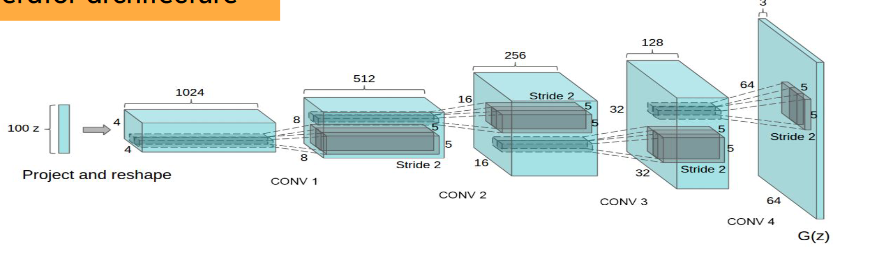
\includegraphics[width=\linewidth]{tikz/DCGAN.png}
    \caption{{\color{red}\colorbox{pink}{Tikz TO-DO}} The figure shows the architecture of the \textbf{Generator} in DCGAN. Multiple Convolutional layers are used in order to produce an high quality image (64x64) starting from a small sampled random vector.}
    \label{fig:DCGAN}
\end{figure}


\subsection{Arithmetic of GAN}

In “Unsupervised Representation Learning with Deep Convolutional Generative Adversarial Networks” the authors explored the latent space for GANs fit on a number of different training datasets, most notably a dataset of celebrity faces. They demonstrated two interesting aspects


Generally speaking, the Generator takes a \textbf{point} from the latent space as input and generates a new image. The latent space itself has no meaning. Typically it is a 100-dimensional hypersphere with each variable drawn from a Gaussian distribution with a mean of zero and a standard deviation of one. Through training, the generator learns to map points into the latent space with specific output images and this mapping will be different each time the model is trained.

This paper showed that, in order to compute the output image, the generator computes vector arithmetic with faces. For example, the Figure \ref{fig:GAN-faces} shows a face of a smiling woman minus the face of a neutral woman plus the face of a neutral man resulted in the face of a smiling man.

In this case, the arithmetic is performed on the $z$ vectors (points in the latent space) corresponding to each resulting faces. Actually on the \textbf{average} of multiple faces with a given characteristic, to provide a more robust result.

Thus,  arithmetic is performed on the mean vectors and creating a
\textbf{vector y}. The center sample on the right hand side is produced by feeding the new vector y with perturbations as input to the generator. 

The results showed that the Generator has some interpolation\footnote{Interpolation means that vectors in latent space can be combined in order to obtain a sample  whose features are a combination of the two} capabilities.

\begin{figure}[!htbp]
    \centering
    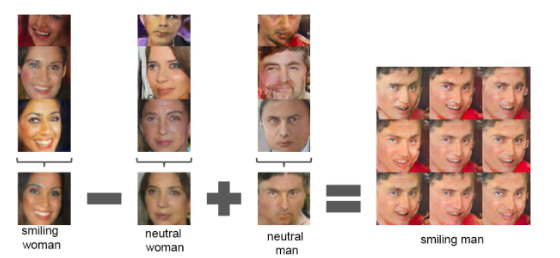
\includegraphics[width=\linewidth]{tikz/Arithmetics of GAN.png}
    \caption{{\color{red}\colorbox{pink}{Tikz TO-DO}} Example of Vector Arithmetic on Points in the Latent Space for Generating Faces With a GAN.}
    \label{fig:GAN-faces}
\end{figure}

\subsection{Evaluate GAN}

It is very had to evaluate a GAN model due to lack of clear methods to evaluate the visual quality of a generated image. The first attempt that was made was using human feedbacks, which of course carries subjectivity and monetary problems.


Furthermore, we are not just interested in the goodness of generated images, but also in looking at the global distribution of the generated samples by GAN, which should be similar to our dataset. Of course, there is no way to directly compute the likelihood of high-dimensional samples (real or generated) or compare their distributions.

To make things easier, we can break down the evaluation problem into two properties: we want to evaluate our GAN on capacity of generating \textbf{recognisable objects} and \textbf{variety of objects} (see figure \ref{fig:inception-score}). Both properties are associated to likelihood (probability). This is computed through the usage of classifier, such as Inception-v3 (pre-trained on ImageNet).  Then, we use its output (probability distribution) to compute the inception score.

\textbf{Inception score}:  the  score is calculated based on the output of a image classification model and it is maximized if:  The entropy of the distribution of labels for the generated images is minimized (\textbf{recognizable}); The predictions of the classification model are evenly distributed
across all possible labels (\textbf{variety}).

However, this metric comes with a overfitting problem: with this method, a GAN that simply memorizes the training data could still score well. If this sentence does not make sense for you, try to think "Why a GAN that genrates very similar samples to my training set should be useful?". Of course such model is not useful at all as it just copy paste seen images. The inception score does not  take into account this problem.


Thus, a better approach is to employ the Fréchet Inception Distance (FID).

\textbf{FID}: the generated samples are passed through a classification network (v3 classifier) and for a choosen layer the activations are computed. Then the metric takes the embeddings of such layer and threats theme as a multivariate normal distributions. We compute the mean and the covariance for both generated samples and real data (also passed into the same layer, extracted embedding and treated as the same distribution) and compare them using the Multivariate Normal Fréchet Distance or Wasserstein-2 distance. However, \textbf{Overfitting problem is not totally avoided.}


\begin{figure}[!htbp]
    \centering
    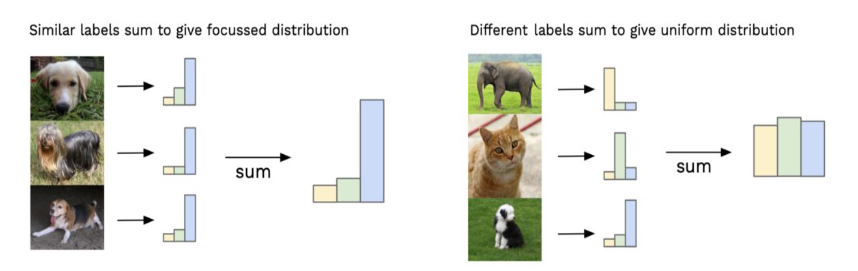
\includegraphics[width=\linewidth]{tikz/Inception score.png}
    \caption{{\color{red}\colorbox{pink}{Tikz TO-DO}} \textbf{Left}: The GAN should produce \textbf{recognisable objects}: if GAN produces picky distributions when it generates images belonging to the same class, this means that each of them are associated to an high likelihood of belonging to that certain class; \textbf{Right}: if we take globally the dataset, the GAN should be able to produce a \textbf{variaty of objects}}
    \label{fig:inception-score}
\end{figure}

\subsection{Mode Collapse}

Mode collapse is one of the most serious issues related to GAN training. It happens when the Generator, instead of capturing all the mode of the target distribution, ends up capturing just one sub mode, i.e. learns just certain area of the target distribution.


\begin{figure}[!htbp]
    \centering
    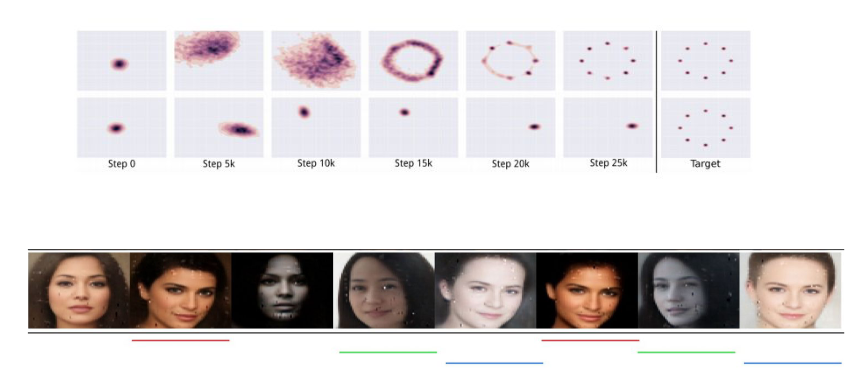
\includegraphics[width=1\linewidth]{tikz/mode collapse.png}
    \caption{{\color{red}\colorbox{pink}{Tikz TO-DO}} The figure shows an example of Mode collapse with faces dataset. The distributions reported above reflects the fact that, instead of learning all the modes of the faces, the generator focuses in just one area (point) of the global distribution. Thus, it generates only asian and female like samples (gnam gnam).}
    \label{fig:mode-collapse}
\end{figure}

\subsection{Losses}

The key concept that a loss function plays in GAN is the following: \textbf{Different losses correspond to different ways to comparing the two distributions}.

We will now analyze 2 different losses in respect of the vanilla GAN.

\subsubsection{LSGAN}

LSGAN is a type of loss function that tries to stabilize the training of a GAN.

The cross entropy is replaced by the \textbf{Least Square Loss}. This leads to better quality generated images (i.e. better IS and FID) and more robust Generators to mode collapse.


\subsubsection{Wasserstein GAN}

This paper tried to modify the loss by using a new way to better matching the dataset and generated samples distributions.

\textbf{Wasserstein distance}: is a metric that matches two distributions with the concept of \textbf{optimal transport}. It measures the minimum cost of transporting mass to convert the data distribution q to the data distribution p. 

\begin{figure}[H]
    \centering
    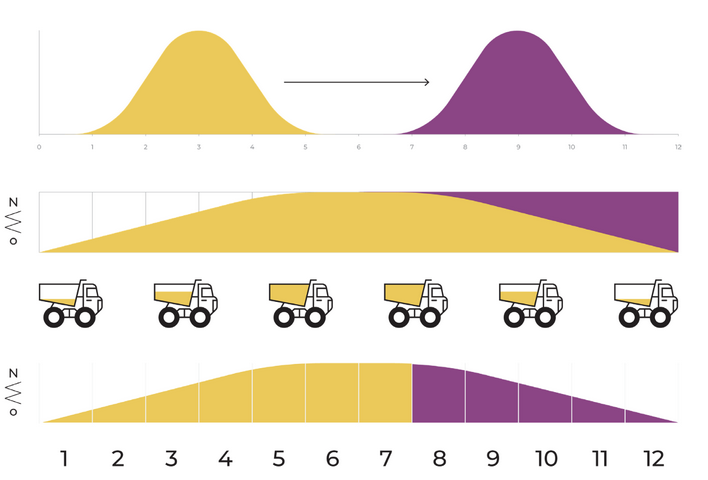
\includegraphics[width=0.75\linewidth]{tikz/WS loss.png}
    \caption{WS loss example}
    \label{fig:WS-loss}
\end{figure}

Wasserstein GAN implemets the idea of matching the two distributions with this distance, which leads to a different cost function that is way better in respect of cross-entropy and Least Sqaure thus leading to a better model. In few words, using the Wasserstein distance provides \textbf{better gradients and more stable training}. 


The most important result was that, if we implement the Wasserstein GAN with DCGAN architecture, it allows us to \textbf{correlate the quality of the sample with the Wasserstein distance value}: if the generated samples improve in quality, the two distributions start matching as the WS distance decreases. This is a big improvement in respect of other GANs. For example, neither DCGAN with the original divergence was able to obtain such property.


However, still the more complex the distance is, the harder the training becomes. 

\begin{figure}[H]
    \centering
    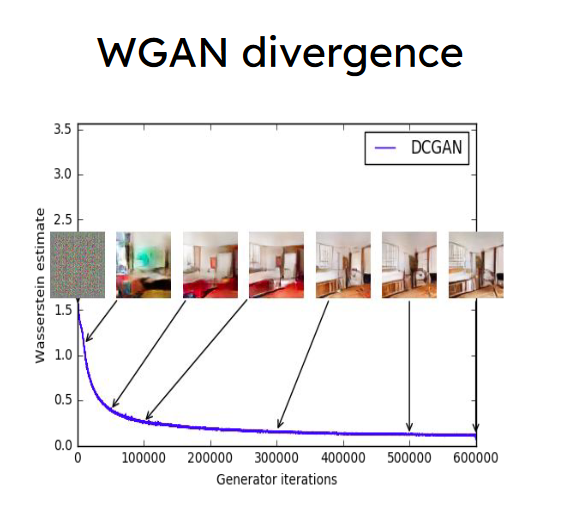
\includegraphics[width=0.75\linewidth]{tikz/WS quality.png}
    \caption{The biggest result of WS distance with DCGAN}
    \label{fig:WS-quality}
\end{figure}



\subsection{Training Tricks}

\subsubsection{Feature matching}

Feature matching is a  regularization technique that addresses the problem that the generator continually seeks to create the most convincing image to deceive the discriminator. As the generator and discriminator constantly adapt to each other’s strategies, the definition of the "best" image keeps changing. This ongoing adaptation prevents the model from converging and often leads to mode collapse.

So the solution is to add a loss for feature matching. It expands the goal from beating the opponent to match features in real images and limits mode collapse.

In other words, instead of focusing in just fooling the discriminator, the new objective requires the generator to generate data that matches the statistics of the real data.  Specifically, we train the generator to match the expected value of the features on an intermediate layer of the discriminator. By training the discriminator we ask it to find those features that are most discriminative of real data versus data generated by the current model.

\begin{figure}[!htbp]
    \centering
    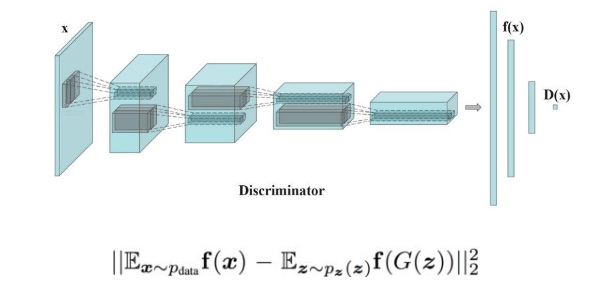
\includegraphics[width=\linewidth]{tikz/feature matching.png}
    \caption{{\color{red}\colorbox{pink}{Tikz TO-DO}} An example of feature matching regularization term.}
    \label{fig:feature-matching}
\end{figure}


 

\subsubsection{Mini-batch discrimination}

With this technique, the discriminator discriminates between whole minibatches of samples rather than between individual samples. This is intended to avoid collapse of the generator.


Specifically, the model computes the similarity of the image x with images in the same batch. Then, it appends the similarity $o(x)$ in one of the dense layers in the discriminator to classify whether this image is real or generated.

If the mode starts to collapse, the similarity of generated images o(x)
increases, making easier for the discriminator to detect the generated images
and penalize the generator.


\begin{figure}[!htbp]
    \centering
    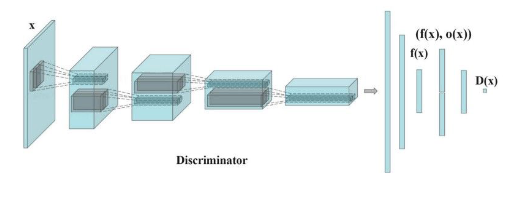
\includegraphics[width=\linewidth]{tikz/Minibatch discrimination.png}
    \caption{{\color{red}\colorbox{pink}{Tikz TO-DO}} Enter Caption}
    \label{fig:mini-batch-discrimination}
\end{figure}

\subsubsection{Virtual batch}

This is a normalization method used for training GANs that extends batch normalization. Regular batch normalization causes the output of a neural network for an input example to be highly dependent on several other inputs in the same minibatch. To avoid this problem in virtual batch normalization (VBN), each example is normalized based on the statistics collected on a reference batch of examples that are chosen once and fixed at the start of training, and on itself. The reference batch is normalized using only its own statistics. VBN is computationally expensive because it requires running forward propagation on two minibatches of data, so the authors use it only in the generator network.


\subsection{Conditional GAN}

As we have seen before, essentially a GAN is composed by two Neural Newtworks. NN can digest arbitrary data structure. This means that a GAN can be transformed to make it able to deal with conditional inputs, such us paired image-label.

\textbf{Conditional GAN} links an input with the associated label. This is useful because allow us to use a GAN with supervised information (for example a photo of a lion along with the label "leon"). The optimization problem does not change, so we can still apply the very same knowledge studied so far.

The main difference is that, in the Generator, the label is just an \textbf{extension} of the latent space $z$. We could append a one-hot enconding vector to $z$. Furthermore, the discriminator will use the label information of real data. This helps to discriminate because, with the given extra information, the Discriminator will be already focused on a specific class.

The loss remains the same as the vanilla one and same previous reasoning hold.

\begin{figure}[!htbp]
    \centering
    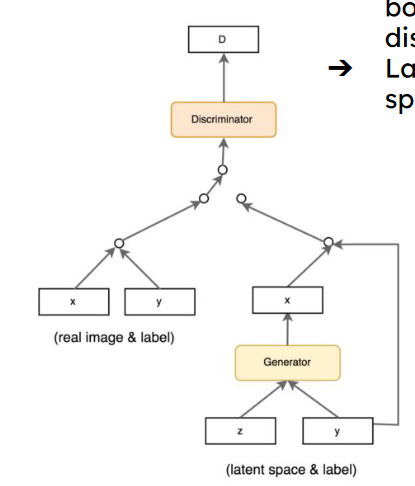
\includegraphics[width=0.5\linewidth]{tikz/conditional gan.png}
    \caption{{\color{red}\colorbox{pink}{Tikz TO-DO}} The architecture of a Conditional GAN}
    \label{fig:conditional-GAN}
\end{figure}


\subsubsection{Image2Image Translation}

This paper is significant because it was the first to present a method for translating one type of pixel representation to another, such as converting a grayscale image to a color image.

To assess this task, the paper introduced PIX2PIX Network. The architecture is nothing new, using a regular Generator and The Discriminator containing many layers. Furthermore, the loss has not changed, comparing the ground image with the generated one.

However, to train this model, we need paired data: for example, if we employ segmentation mask, for each segmentation we would need a real associated image.
 

\begin{figure}[!htbp]
    \centering
    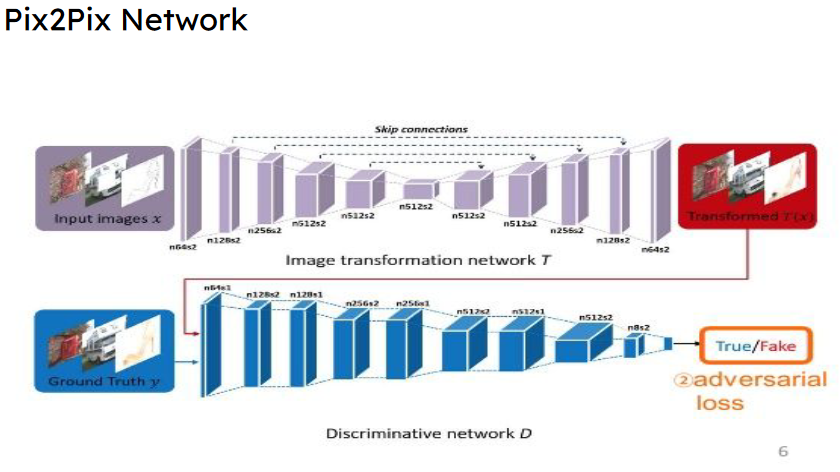
\includegraphics[width=\linewidth]{tikz/image2image.png}
    \caption{{\color{red}\colorbox{pink}{Tikz TO-DO}} PIX2PIX architecture}
    \label{fig:image-2-image}
\end{figure}


\subsubsection{Cycle GAN}

It is another work that implements the concept of Image2Image translation \textbf{overcoming the limitation of having paired samples}.

For example, if we have a collection of natural images and a collection of Monet paintings, which are not paired with each other, we can implement \textbf{cross-domain transfer} using a CycleGAN architecture.

CycleGAN consists of \textbf{three networks}, namely the Discriminator, Generator and Translator networks: 

\begin{itemize}
    \item \textbf{Translator}: this network is used to "translate" an image from one domain (natural domain) to the other (painting domain).
    \vspace{5 pt}

    \item \textbf{Discriminator}: it is trained to detect if the translated image could came from the target domain. Furthermore, the translated image is then reconstructed to its original domain and the Discriminator is employed to check its correctness.
    \vspace{5 pt}

   \item \textbf{Generator}: the network  takes the translated image and converts it back to the original domain. 
\end{itemize}



This peculiar architercute leads to a modification on the training loss: besides the classical loss of vanilla GAN, an additional one is needed to ensures that the reconstructed image is similar to the original natural image,   \textbf{ reconstruction loss} (L1 loss).


The flow is applied in both directions, meaning that we first translate and reconstruct an image from one domain (from natural to Van Gogh), then we do the same for the other domain (from VanGogh to natural) by inverting the architecture. The parameters are shared among the two iterations. 




\begin{figure}[!htbp]
    \centering
    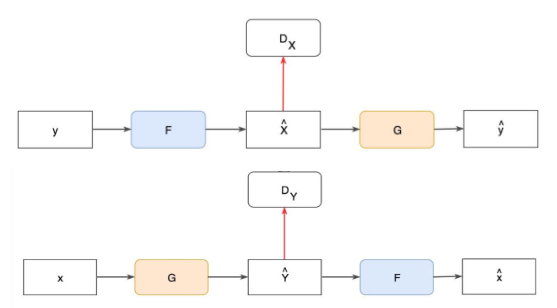
\includegraphics[width=\linewidth]{tikz/Cycle GAN.png}
    \caption{{\color{red}\colorbox{pink}{Tikz TO-DO}} The image shows the architecture of Cycle GAN, where $y$ is an image from Natural domain, $x$ is from Van Gogh domain, $F$ is the Translator network, $\hat{x}$ is the translated sample from natural to Van Gogh, $\hat{Y}$ is the generated sample from Van Gogh to Natural domain}
    \label{fig:cycle-GAN}
\end{figure}

\subsection{Progressive GAN}

This type of model implemented the idea of progressively growing the Generator and the Discriminator during the training with the final scope of \textbf{generate high-quality images}.

The advantage is that, at each step, both networks take into advantages the parameters learned during the previous step (see figure \ref{fig:progressive-GAN}). With this slow training, we imposes the GAN to learn the structural contents first and iteratively  use it to add details. This allows the model to generate high-quality images.


The training requires to start with a base model with G and D trained with small images and once the training stabilizes new blocks of layers are added which are capable of taking in larger images, and the model is trained again. This is repeated until the desired image size is achieved.

\begin{figure}[!htbp]
    \centering
    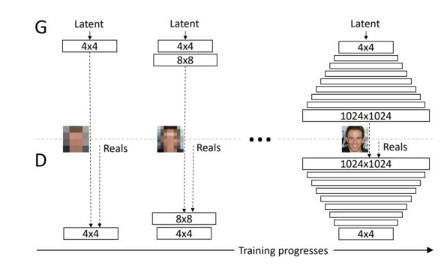
\includegraphics[width=\linewidth]{tikz/Progressive GAN.png}
    \caption{{\color{red}\colorbox{pink}{Tikz TO-DO}} Progressive GAN architecture}
    \label{fig:progressive-GAN}
\end{figure}


\subsection{Style GAN}

This model modified a bit some parts of the Generator network, making it able to capture the \textbf{style attributes} of an image (pose, type of hair, the smile form, ecc...). Furthermore, it also allow to change them in a stochastic fashion (using random noise).


The model replaced the conventional upsampling with bilinear sampling. We need some form of style vector, which is obtained by passing some latent representation to 8 FC layers. The vector recives information thanks to \textbf{Instance Normalization}.

We operate to instance level, so we maintain information of each instance: this type of normalization process allows to remove instance-specific contrast information from the content image, producing statistics ($\mu$ and $\sigma$) that contains information related to the style of the image. 

Instance normalization is applied to different levels to capture different style factors. Those are re-integrated when the synthetic image is outputed.


\subsection{Drag GAN}
DragGAN is a recent invention in GAN models that enables the editing of images in a user-friendly manner through a simple point-and-drag methodology. 

The user starts by defining a couple of \textbf{pairs of handle} and \textbf{target points}, which represent the positions of parts of the image to be manipulated.  The objective here is for the user to be able to drag portions of the image from the position of the handle points to the position of the target points. Optionally, the authors also provide the user with the choice of selecting a region of the image which can be moved as a part of this manipulation exercise. 

The optimization process is broken down into 2 parts:

\begin{enumerate}
    \item \textbf{Motion Supervision}: This is the first step that involves optimizing for a loss function that causes the handle points to move toward the target points.
    \vspace{1 pt}
    \item \textbf{Point Tracking}: This is the second step that updates the handle points to track the object itself so that the handle points are updated after the motion supervision step and the focus is still the same manipulations as initially defined by the user. This step is achieved using nearest neighbor interpolation.

\end{enumerate}

\begin{figure}[!htbp]
    \centering
    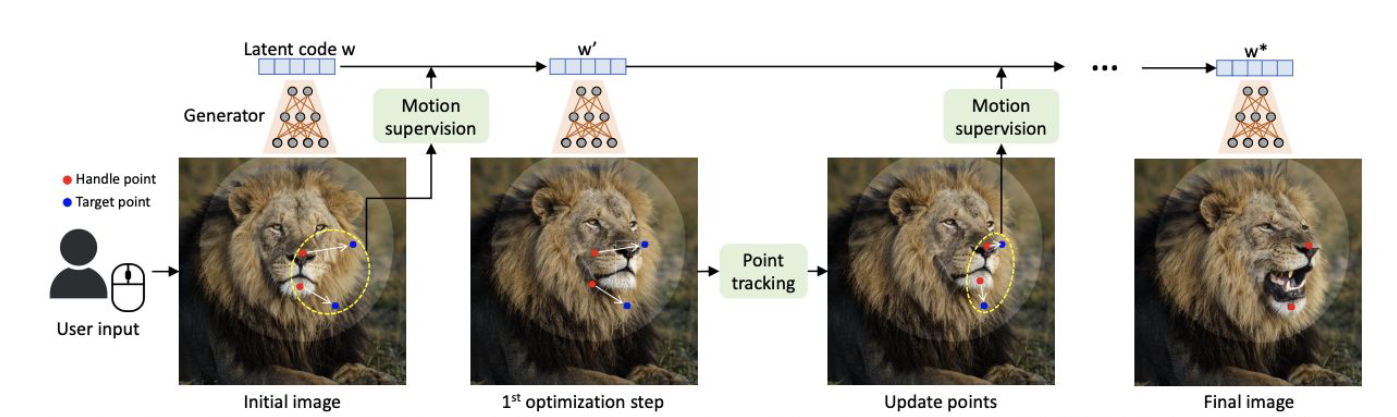
\includegraphics[width=1\linewidth]{tikz/DRAG GAN.png}
    \caption{{\color{red}\colorbox{pink}{Tikz TO-DO}} The image above summarizes the approach of DragGAN. (\textbf{1}). The user defines pairs of points on the original image, the red points signify the handle point and the blue points signify the target point. Optionally, the user can also define a specific area on the image that can move during the process of image editing; (\textbf{2.}) The first step, motion supervision is performed on the learned image representations of the Generator; (\textbf{3.}) The second step is performed on the image produced after point tracking to update the position of the handle points. (\textbf{4.}) Then, this pattern of the first step followed by the second step is repeated until the final image is produced.}
    \label{fig:drag-gan}
\end{figure}

\section{Explitic Density Estimantion}



\subsection{Autoencoder}

Auto-encoder is a model that is trained on unlabeled data and is used to map the input data to a reduced feature representation before reconstructing it  from that feature representation.

\begin{figure}[!htbp]
    \centering
    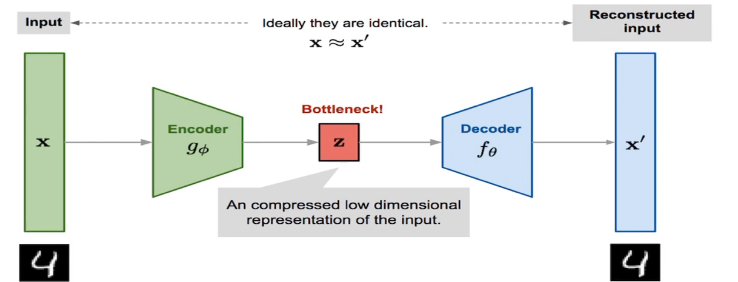
\includegraphics[width=1\linewidth]{tikz/Autoencoder.png}
    \caption{{\color{red}\colorbox{pink}{Tikz TO-DO}} The figure shows the tipical workflow and architecture of an Autoencoder used for image reconstruction: given an image, the autoencoder must reconstruct the same image.}
    \label{fig:autoencoder}
\end{figure}

In order to do that, the input is fed into the \textbf{Encoder}, which can be a Linear + nonlinearity (sigmoid), a Deep fully-connected network, or the defacto standar is ReLU CNN (for images). The Encoder compresses the image into a lower dimensional latent representation $z$, often called \textbf{bottleneck}. This layer contains only the \textbf{most important features} extracted from the input. The \textbf{Decoder} module, which is a symmetric network in respect to the encoder, then decompress the latent representation $z$ into the input dimension producing a similar sample $x^{'}$.  The generated sample is then compared to the original input $x$ by computing a reconstruction loss function, the \textbf{L-2 Norm}.

$$ L(\theta, \phi) = \|x-\hat{x}\|^2 $$

The training aims at finding the wieghts of the encoder and decoder that minimize the loss function. As we can see, the L-2 norm depends on parameters that define the two modules: \textbf{Encoder} needs to better extract important features from the input; \textbf{Decoder} needs to better decompress the latent compressed features. These parameters refers to the NNs used to construct the encoder and decoder.

After training, the decoder part is thrown away and the encoder can be used to initialize a supervised model, predicting labels from the  feature space $z$.

The reason why Autoencoders learn the lower $z$ (latent represnetation/bottleneck) from a higher-dimensional data $x$ (image) is for capturing the most important parts of the input image. Keeping the bottleneck layer small forces the autoencoder to learn an intelligent representation of the data. Another way to force the autoencoder is adding random noise to its inputs and making it recover the original noise-free data (\textbf{Denoising Autoencoders}).


\begin{figure}[!htbp]
    \centering
    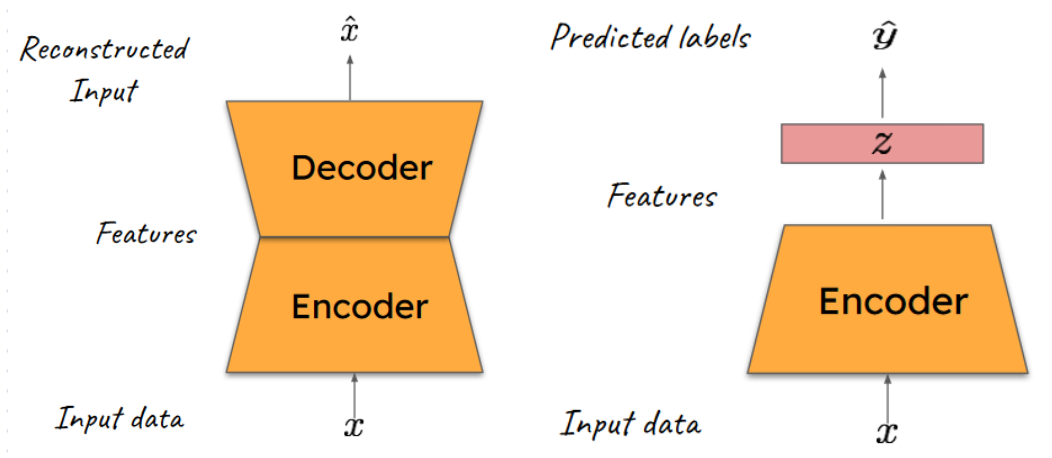
\includegraphics[width=\linewidth]{tikz/Autoencoders.png}
    \caption{{\color{red}\colorbox{pink}{Tikz TO-DO}} \textbf{Left}: the figure shows a global view of the autoencoder architecture, where features represents the bottleneck layer and it is essentially a vector; \textbf{Right}: the figure shows how an autoencoder can be use for initiating a supervised model.}
    \label{fig:autoencoder}
\end{figure}

\subsubsection{Regression on Decoder structure}


As the Decoder is symmetric to the Encoder (mirroring structure), which is a CNN, it is usually implemented with transposed Convolutional Layers.

\textbf{Transposed Convolutional Layer}: this layer is usually carried out for upsampling i.e. to generate an output feature map that has a spatial dimension greater than the input feature map. Just like the standard convolutional layer, the transposed convolutional layer is also defined by the \textit{padding} and \textit{stride}. They are defined using the values used by the encoder.

Implementing a transposed convolutional layer can be better explained as a 4 step process:

\begin{enumerate}
    \item \textbf{Step 1}:  Calculate new parameters $z$ and $p^{'}$
    \item \textbf{Step 2}: Between each row and columns of the input (the features in the bottleneck layer), insert $z$ number of zeros. This increases the size of the input to $(2*i-1)x(2*i-1)$
    \item \textbf{Step 3}: Pad the modified input image with $p^{'}$ number of zeros
    \item  \textbf{Step 4}: Carry out standard convolution on the image generated from step 3 with a stride length of 1
\end{enumerate}

 \begin{figure}[!htbp]
     \centering
     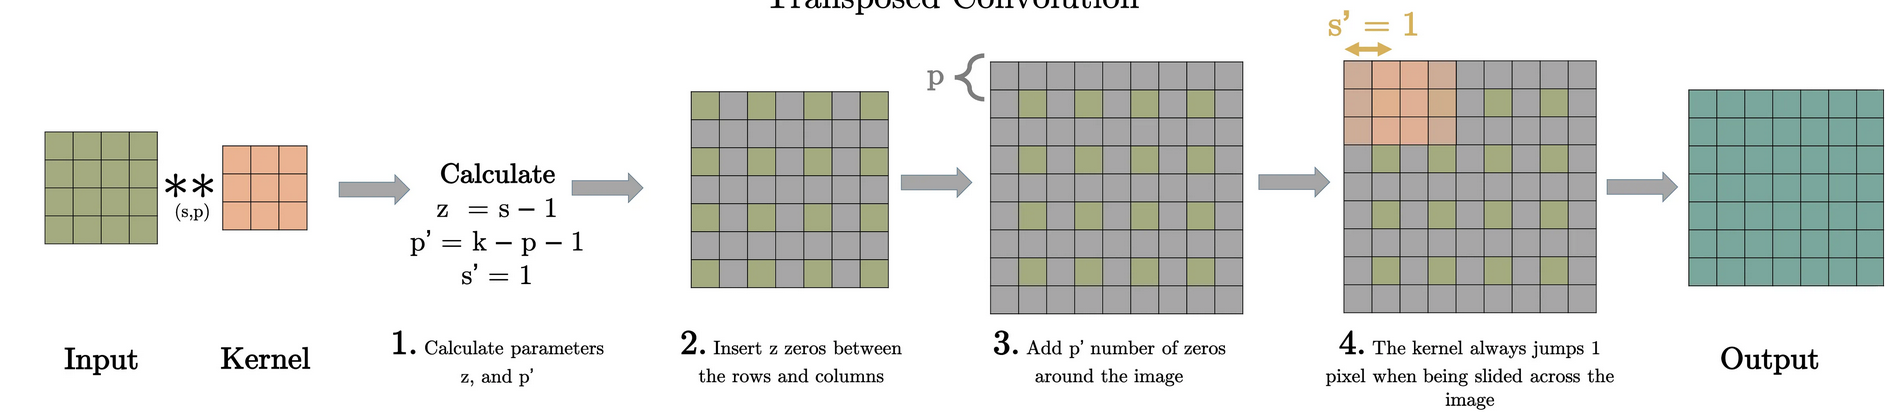
\includegraphics[width=1\linewidth]{tikz/Transposed Convolution.png}
     \caption{{\color{red}\colorbox{pink}{Tikz TO-DO}} Transposed Convolution, Image By Author}
     \label{fig:transposed-convolution}
 \end{figure}



\subsection{Variational Autoencoders}

To get a general intuition of why we need VAE and why they are different from standard AE, let's use the following example:

Let's say we want to develop an open world game. Through an Autoencoder, we would like to learn latent features of objects in our world, for example plants, and take \textbf{random sample} from the latent space in order to generate an \textbf{unique variation}, i.e. unique plant. For the sake of simplicity, taking random sample means to sample x values from a latent space distribution (i.e multivariate normal random variable), where each values corresponds to an attribute of the object.  For example, if we want to generate a plausible variation of plant z by modifying the colour and the pedal width, we would first learn  the corresponding latent features (i.e univariate normal random variables) in the latent space (i.e. multivariate normal random variable) representing the two attributes of plant x, and interpolate them, allowing us to sample these values from a continuous sequence.

However, Standard autoencoder will learn to represent the input (plant) \textbf{just in a compressed form} (the bottleneck). Therefore, the latent space is not \textbf{continuous} and it will not allow any type of \textbf{interpolation}, thus sampling. Autoencoders are only able to \textbf{replicate the input coming from the same dataset}.

VAEs enhance traditional autoencoders by learning distributions for latent features (e.g., petal width, color as univariate normal distributions). By sampling these distributions and decoding, they generate \textbf{unique images} with \textbf{similar} characteristics to the dataset ($p(x|z)$). VAEs create a \textbf{continuous latent space} that allows easy sampling and interpolation, generating new samples similar to the input, whose characteristics are different from the one in the training set.


\begin{figure}[!htbp]
    \centering
    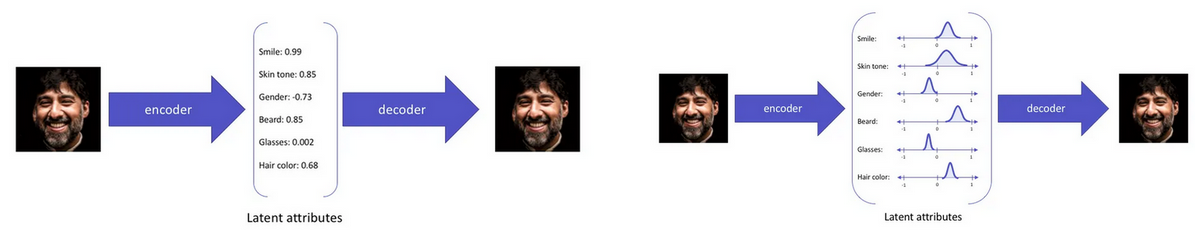
\includegraphics[width=1\linewidth]{tikz/VAE example.png}
    \caption{{\color{red}\colorbox{pink}{Tikz TO-DO}} \textbf{Left}: the figure shows the latent attributes learnt by a standard AE. While they explain the image and can be used in reconstructing the image from the compressed latent space, they cannot be used for probabilistic modelling; \textbf{Right}: The  figure shows the latent attributes learnt by a VAE.  They are continuos and they can be sampled from the latent distribution formed.}
    \label{fig:VAE-example}
\end{figure}

To better explain this type of model, let's remind that it belongs to \textbf{explicit density estimation} family so, instead of having a network that measures the distance among two distribution and instead of indirectly estimate the distribution of our dataset ($p_{model}(x))$, VAE uses a direct approach: the model  estimates the likelihood function for the dataset sample $p_{\theta}(x)$. This estimation problem can be re-written in its integral form:

$$p_{\theta}(x)=\int_{} p_{\theta}(z)p_{\theta}(x|z)dz$$

where $z$ corresponds to the latent representation vector of our training data. 

The formula represents a likelihood function, thus we would like to learn the parameters $\theta$ that maximize it, i.e. such that generated data fit training data.

However, we cannot  directly do this because the likelihood is mapped through $z$ which, as stated above, is a \textbf{latent representation} that we have to learn from our training samples and not the samples themeself (quick reminder: the likelihood function is usually optimized over the data, that in this case are represented by their latent features). Hence, we do not have direct access to data we are integrating over.


Let explain this issue by breaking down into pieces the formula. We can clearly see that it implements two probability distributions: $p_{\theta}(z)$ (\textbf{prior distribution}) represents the latent space; $p_{\theta}(x|z)$ represents the Decoder itself, as it samples $z$ from the latent space distribution $p_{\theta}(z)$ and transform it into a sample $x$ that belong to a complex one distribution that should be similar to training data's ones.


As the Decoder samples from the prior distribution, the latent space should be a simple probability distribution to facilitate this process. Therefore, the latent space is a \textbf{Multivariate Gaussian}.


However, in principle we are not able to directly produce $p_{\theta}(z)$ because it is extracted from training data. \textbf{This is the source of the integration problem}.

\begin{figure}[!htbp]
    \centering
    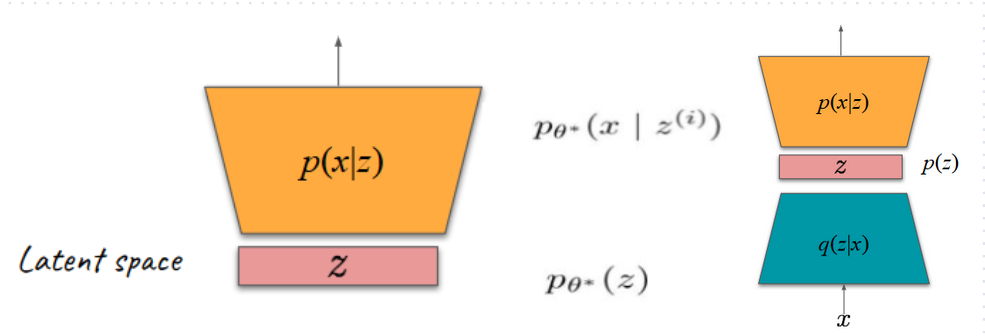
\includegraphics[width=\linewidth]{tikz/VAE posterior.png}
    \caption{{\color{red}\colorbox{pink}{Tikz TO-DO}} The overall image depicts the entire process. In short, our goal is to learn how to generate data, $x$, from our latent variables, $z$. This requires learning $p(z \text{|} x)$. To achieve this, we use the KL divergence to approximate the true posterior probability, which cannot be computed directly using Bayes' theorem. \textbf{Right}: We can choose a simple prior $p(z)$, such as a Gaussian distribution. The conditional probability $p(x∣z)$ is complex (generates the image) and is represented by a decoder neural network. \textbf{Left}: The additional probabilistic encoder}
    \label{fig:VAE-posterior}
\end{figure}

We could obtain $p_{\theta}(z)$ by using the Bayesian theorem. However, another problem arises when we try to compute the posterior probability distribution $p_{\theta}(z|x)$, because the denominator is intractable:

$$p_{\theta}(z|x)= \frac{p_{\theta}(x|z)p_{\theta}(z)}{p(x)}$$

In this context, $p_{\theta}(z|x)$ represents the distribution of the latent space extracted from the given input.

The solution to this dilemma is to use an auxiliary neural network, the \textbf{Encoder}, which will be trained to be able to map the input image into the   latent space, $q_{\phi}(z|x)$. By doing so, it approximates the posterior distribution $p_{\theta}(z|x)$. Hence, the encoder \textbf{does not provide a global solution to the optimization problem but just a proxy}: it will provide a lower bound of the data likelihood.

As described in the gaming example, instead of compressing the latent space, the encoder should maps input to its feature distribution functions / latent space distribution $q_{\phi}(z \text{∣} x)$, allowing continuous values. This enables the probabilistic decoder to sample attribute values from each latent variable's distribution, and use the resulting vector to reconstruct a new image $p_{\theta}(x∣z)$. 

\begin{figure}[!htbp]
    \centering
    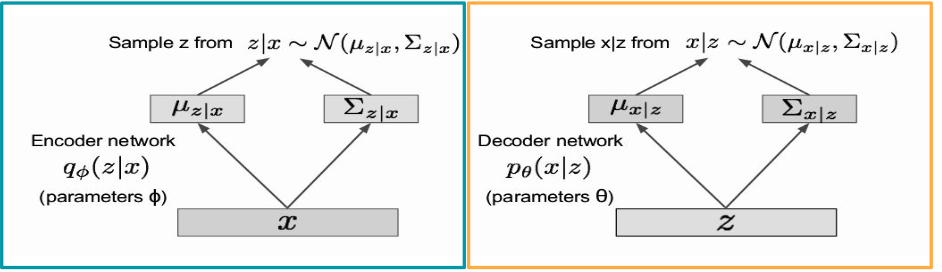
\includegraphics[width=1 \linewidth]{tikz/VAE encoder-decoder.png}
    \caption{{\color{red}\colorbox{pink}{Tikz TO-DO}} Since we are modeling probabilistic generation of data, encoder and decoder networks are probabilistic.}
    \label{fig:VAE-pro-structure}
\end{figure}


So far we have seen the the main changes introduce by VAE in respect of standard AE, which are the \textbf{probabilistic design} of both Encoder and Decoder. This design is needed because we impose the model to learn a latent space constrained in a certain probability distribution, the Gaussian.  


From figure \ref{fig:VAE-pro-structure} we can see that both Encoder and Decoder are described by their own parameters, respectively $\phi$ and $\theta$. The Encoder will learn $\mu$ and $\sum_{}$ associated with the Gaussian distribution of the latent space $z$. The Decoder learns $\mu$ and $\sum_{}$ of the generating distribution $x|z$ (which should be as close as the dataset).



The object function can be derived as follows, applying the log likelihood and multiple transformations:


\begin{equation} \label{eq: VAE-derivation}
\begin{aligned}
log p_{\theta}(x) &= E_{z \sim q_{\phi}(z|x)}\left[ \log p_{\theta}(x) \right]\\
&=E_{z }\left[ \log \frac{p_{\theta}(x|z) p_{\theta}(z)}{p_{\theta}(z|x)} \right]  \text{  bayesian rule applied} \\
&=E_{z }\left[ \log \frac{p_{\theta}(x|z) p_{\theta}(z)}{p_{\theta}(z|x)} \frac{q_{\phi}(z|x) }{q_{\phi}(z|x)}\right] \text{  multiply by constant} \\
&=E_{z }\left[ \log p_{\theta}(x|z) \right] - E_{z} \left[ \log \frac{q_{\phi}(z|x)}{ p_{\theta}(z)}\right] + E_{z} \left[ \log \frac{q_{\phi}(z|x)}{p_{\theta}(z|x)} \right] \\
&=E_{z }\left[ \log p_{\theta}(x|z) \right] - D_{KL} \left[ q_{\phi}(z|x)|| p_{\theta}(z)\right] + D_{KL} \left[ q_{\phi}(z|x)||p_{\theta}(z|x) \right] 
\end{aligned}
\end{equation}


Form equation \ref{eq: VAE-derivation}, the third term is left out as we cannot compute it as we do not have access to $p_{\theta}(z|x)$ (remember, the encoder \textbf{approximates} the posterior distribution). However, this term is always a positive number as it is computed by the KL divergence and this allows us to approximate the likelihood to a lower bound.

\textbf{KL divergence}: The KL divergence is a measure of how similar two probability distributions are; if they are the same, the divergence is zero, and if it is a positive number, the two distributions are different. 

\begin{equation}
    L(\phi, \theta) = E_{z }\left[ \log p_{\theta}(x|z) \right] - D_{KL} \left[ q_{\phi}(z|x)|| p_{\theta}(z)\right]
\end{equation}

We are left with two remaining terms: the first is the \textbf{reconstruction loss}. This term is applied to the decoder in order to train it to generate something meaningful when sampling from the latent representation in respect to the input data.

The second one can be computed in close form as it involves computing the KL divergence between  two gaussian distributions and it used for the encoder (because it tries to approximate the prior distribution which is a gaussian). This term is often called \textbf{regularizer} as it imposes the latent space to behave to match a gaussian distribution.


The combination of these two factors allows the latent space to be smooth, ensuring smooth interpolation among the latent representations of samples without any gaps. This forces the encoder to produce a Gaussian distribution that is close to the prior.

\begin{figure}[!htbp]
    \centering
    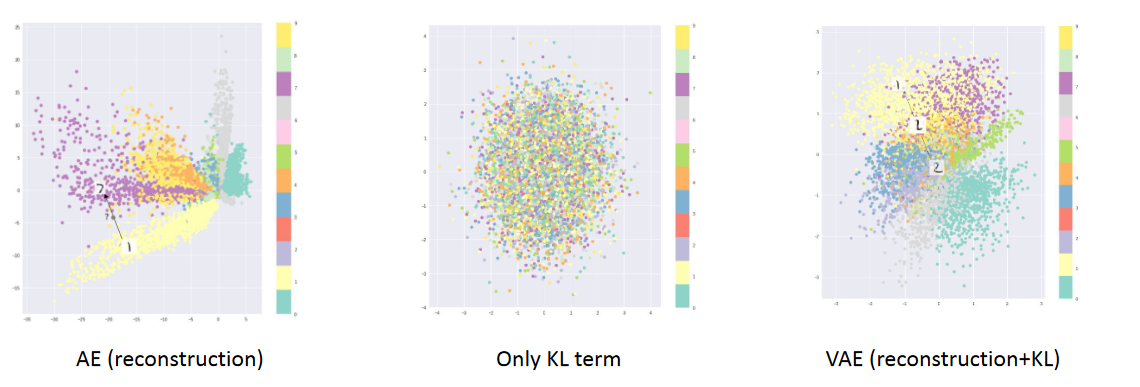
\includegraphics[width=\linewidth]{tikz/VAE latent spaces.png}
    \caption{{\color{red}\colorbox{pink}{Tikz TO-DO}} The figure compares three different latent spaces. \textbf{Left}: is obtained when only the reconstruction loss is used, like in traditional Autoencoders. We do not have controll over the latent space distribution; \textbf{Center}: is obtained when only regularizer term is used. In this case, the model will end up learning a narrow distribution for each different type of sample; \textbf{Right}: is obtained when both terms are used. Optimizing these two terms jointly allows the latent space to fit the data well and be smooth, resembling a Gaussian distribution. Consequently, the latent space behaves appropriately.}
    \label{fig:VAE-latent-spaces}
\end{figure}



Another difference between VAEs and Autoencoders is that Autoencoders are not inherently generative models because there are no constraints on the latent space to ensure it behaves in a specific way (see figure \ref{fig:VAE-latent-spaces}). If we train an autoencoder, take the latent space, and add some noise, the decoder will produce meaningless results. This is because, during training, there was no mechanism to enforce the latent space to behave in a structured manner.

\paragraph{Backpropagation issue}

When optimizing, we need to alternate optimization of both parameters. However, when we try to take the derivative in respect of $\phi$, problems arises.



This is linked to the prior probability. Remeber that we have assumed the prior $z$ to be a \textbf{multivariate Gaussian distribution}, and we aim to build a parameterized distribution close to it, which parameters are the latent $\mu$ and $\sum_{}$. We then sample from it a vector that is fed to the decoder, which then proceeds to reconstruct the input from the sample points.

While this seems easy in theory, it becomes impossible to implement because backpropagation cannot be defined for a random sampling process performed before feeding the data to the decoder.

To get by this hurdle, we use the \textbf{reparameterization trick}.

\textbf{Reparametrization trick}: In the reparameterization trick, we randomly sample a value $\epsilon$ from a standard Gaussian and then scale this by the latent distribution variance $\sigma$ and shift it by the mean $\mu$ of the same.

$$z = q_{\phi}(\epsilon, x) \text{ with } \epsilon \sim N(0,1)$$


which in close form is 

$$q_{\phi}(\epsilon, x) = \mu_{}(x) + \epsilon \sum_{} (x)$$

And still $z$ is distributed as a multivareate normal distribution $$z \sim N(\mu(x), \sum_{} (x))$$ 


The reparameterization trick is a little esoteric, but it basically says that I can write a normal distribution as a mean plus some standard deviation, multiplied by some error. This means that when differentiating, we are not taking the derivative of the random function itself, merely its parameters.

Now, we have left behind the sampling process as something done outside what the backpropagation pipeline handles, and the sampled value $\epsilon$ acts just like another input to the model, that is fed at the bottleneck.




\begin{figure}[!htbp]
    \centering
    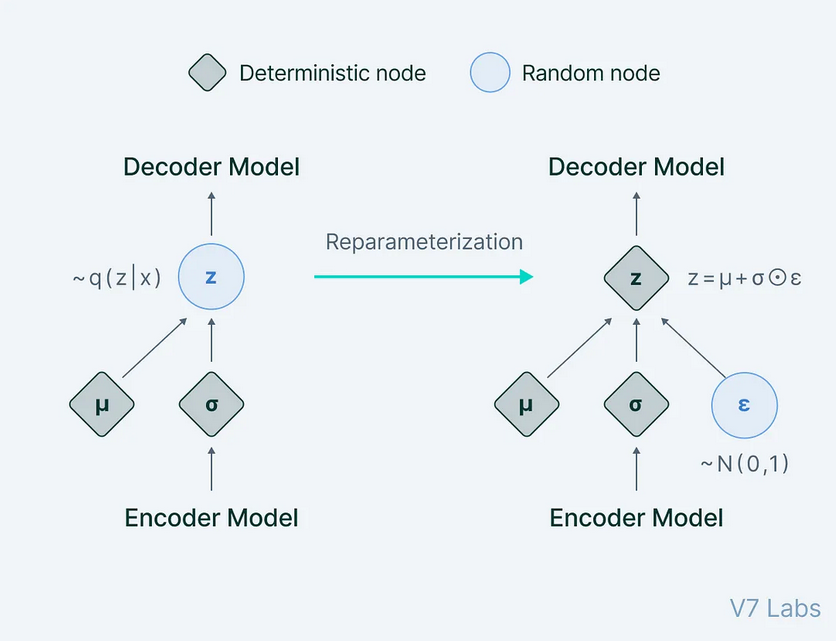
\includegraphics[width=\linewidth]{tikz/VAE training.png}
    \caption{{\color{red}\colorbox{pink}{Tikz TO-DO}} The reparametrization trick applied to the prior distribution}
    \label{fig:VAE-training}
\end{figure}


\paragraph{Data Generating Procedure}

During this process, the model just samples from $z$ and pass it to the decoder network (see Figure \ref{fig:VAE-example}).

For example, looking at Figure \ref{fig:VAE-generating-process}, we want to generate the number ‘2’, so it generates the value 2 from the latent variable centroid. However, we may not want to generate the same looking ‘2’ every time, as in our video game example with plants, so we add some random noise to this item in the latent space, which is based on a random number and the ‘learned’ spread of the distribution for the value ‘2’. We pass this through our decoder network and we get a 2 which looks different to the original.

 Parameters that look similar are clustered together in the latent space, and are not spaced arbitrarily. This is illustrated in the figure below. We see that our values of 2’s begin to cluster together, whilst the value 3 gradually becomes pushed away. This is useful as it means the network does not arbitrarily place characters in the latent space, making the transitions between values less spurious.


\begin{figure}[!htbp]
    \centering
    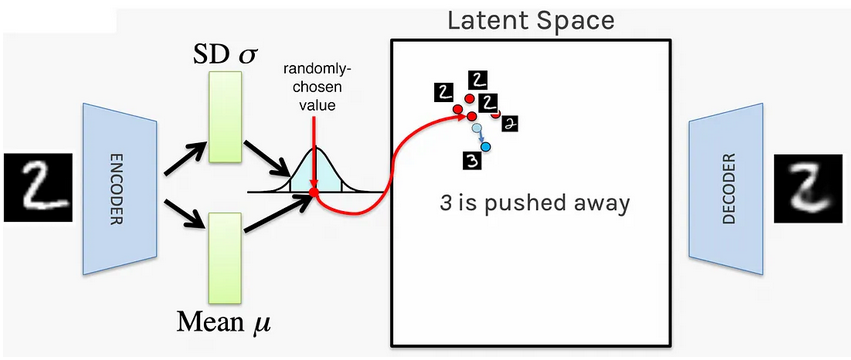
\includegraphics[width=\linewidth]{tikz/VAE generating process.png}
    \caption{{\color{red}\colorbox{pink}{Tikz TO-DO}} Example of data generating process for MINST dataset}
    \label{fig:VAE-generating-process}
\end{figure}


\begin{figure}[!htbp]
    \centering
    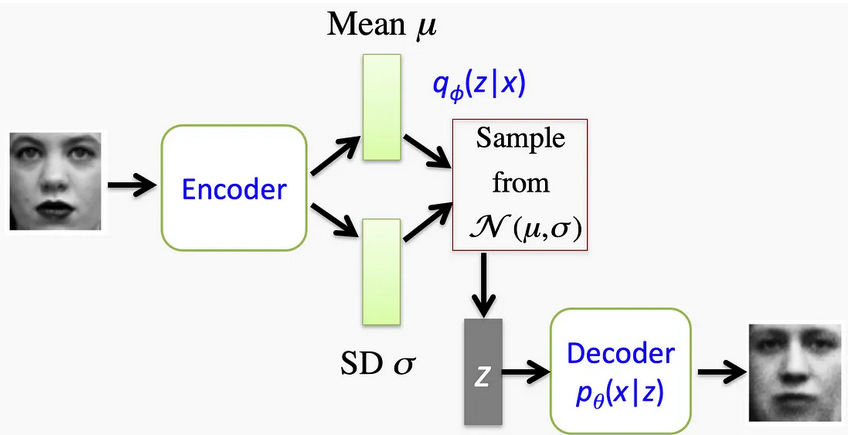
\includegraphics[width=\linewidth]{tikz/VAE entire process.png}
    \caption{{\color{red}\colorbox{pink}{Tikz TO-DO}} The image shows an overview of the entire network architecture. We train the autoencoder using a set of images to learn our mean and standard deviations within the latent space, which forms our data generating distribution. Next, when we want to generate a similar image, we sample from one of the centroids within the latent space, distort it slightly using our standard deviation and some random error, and then pass this through the decoder network. It is clear from this example that the final output looks similar, but not the same, as the input image.}
    \label{fig:VAE-entire-process}
\end{figure}


\begin{comment}


\paragraph{Latent vector}

As in the standard approach, the latent vector $ z $ encapsulates essential features (attributes) of a given input. Each attribute is represented by a \textbf{latent variable}, corresponding to a real feature of the object and their values  are derived from the original sample $x$. These attributes, as implied by the term \textbf{latent}, cannot be directly measured. An example is the age attribute shown in Figure \ref{fig:VAE-example}.

\textbf{Qeustion n.1}: How are these latent variables' values computed by the model?


The partial answer lies in the fact that the architecture has changed, now employing a probabilistic approach (Figure \ref{fig:VAE-architecture}). Specifically, the architecture consists of two modules:  the \textbf{Probabilistic Encoder}, represented by $q_{\phi}(z|x)$, and the \textbf{Probabilistic Decoder}, represented by $p_{\phi}(x|z)$. 

\textbf{Answer to question n.1}: 

Instead of compressing the features, the encoder maps the input into the feature distribution function $q_{\phi}(z|x)$, allowing the values to be continuous. 


This allows the probabilistic decoder to sample attribute values from each latent variable's distribution, using the resulting vector to reconstruct a new image with the conditional probability $p(\hat{x}|z)$, where $\hat{x}$  is the new sample.



Furthermore, the encoder divides the features size of $x$ into two parts, the mean $\mu$ and the standard deviation $\sigma$. Subsequently, they are join toghether into $z$ representation, by a linear transformation that involves $\mu$,  multiplying $\sigma$ with a random sample sampled from a standard normal distribution $\sim N(0,1)$.



\begin{figure}[!htbp]
    \centering
    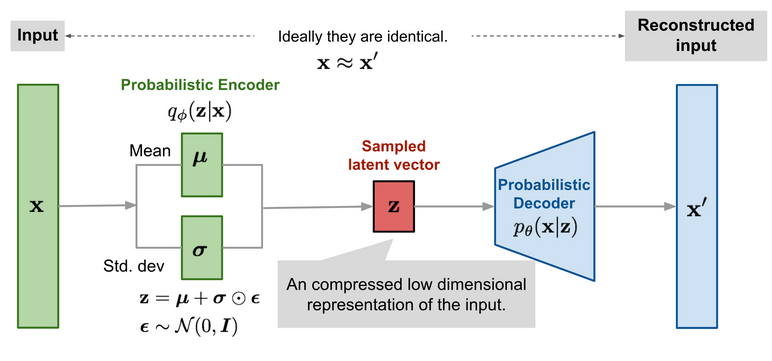
\includegraphics[width=1\linewidth]{tikz/variational autoencoder.png}
    \caption{{\color{red}\colorbox{pink}{Tikz TO-DO}} Enter Caption}
    \label{fig:VAE-architecture}
\end{figure}



\textbf{First summarized difference}:

Using a VAE, we \textbf{represent each latent attribute for a given input as a probability distribution}, unlike standard autoencoders. For example, given an image of a man (Figure \ref{fig:VAE-example}), a standard AE fixes the smile feature, while a VAE learns a probability distribution for the smile. During decoding, we randomly sample from this distribution for each latent variable, generating a vector used by the decoder to create a new unique image. \textbf{The features of the generated image will belong to the same distribution as the input, but will be different from the samples in our dataset}.

Hence, that is why  we aim to construct our encoder model as a probabilistc one. It must be able to output a \textbf{range of possible values} for each latent attributes from which we will randomly sample to feed into our decoder model.


A visual explanation is provided in Figure \ref{fig:VAE-prob}. If we sample green and orange features from the smile probability distribution, they are close to each other in the latent space. Consequently, when these latent vectors are fed into the decoder, the generated images will look similar to the original one because their vectors are similar, and vice versa.


\begin{figure}[!htbp]
    \centering
    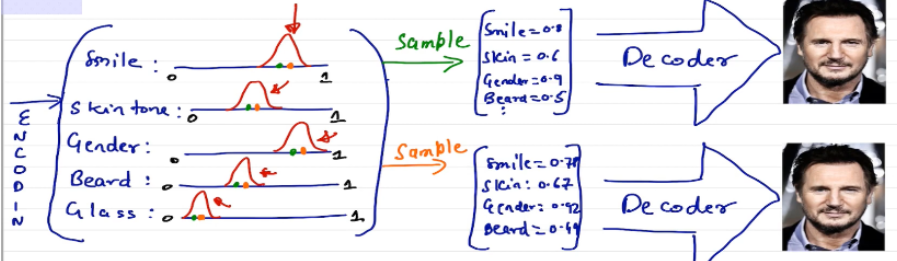
\includegraphics[width=1\linewidth]{tikz/VAE latent space.png}
    \caption{{\color{red}\colorbox{pink}{Tikz TO-DO}} Enter Caption}
    \label{fig:VAE-prob}
\end{figure}




Before diving into the mathematical part and defining the training Loss, we still miss a crucial aspect for easily understanding VAE, which is the goal they try to pursue!

\paragraph{Goal}

\underline{Let us first state it in probabilistic fashion}:

The goal of VAE is to find a distribution $q_{\phi}(z|x)$ (the encoder) of some latent variables $z$ (latent attributes) from which we can sample from $z \sim q_{\phi}(z|\underline{x}) $ to generate a new samples $x^{'} \sim p_{\theta}(x^{'} |z)$ (see figure \ref{fig:VAE-architecture} to better understanding to whom this probability functions refer to). 

We want to stress the keyword \textbf{new} because, when we feed the sampled latent vector $z$ (containing the sampled values of each latent variable)  into the probabilistic decoder, it generates a sample $x^{'}$ that is not present within our dataset but \textbf{still}  has the same distribution of the original sample x.

\underline{Now, let's explaint this concept in a not probabilistic way}:

A VAE ensures that encodings from a known probability distribution can be decoded into reasonable objects, \textbf{even if they are the same of the actual image}, as they share the same probability distribution.

Traditional autoencoders cannot perform this task since they learn the "probability distribution" of a \textbf{restricted domain}. For instance, an autoencoder trained on the MNIST dataset will output random noise when given an image from a different dataset because the decoder cannot recognize the different probability distribution of the latent representation.

VAEs, instead of producing single-value encodings, produce a probability distribution function for \textbf{each encoding} (see Figure \ref{fig:VAE-example}). The decoder then samples from these distributions to cluster the images.





\paragraph{Loss Function}

Welcome to the madness! In this subsection we will describe the loss object of VAE in a problem-solution flow manner. Why such approach? Because many problems are linked to the probabilistic style of the two modules. 

Let's start with first defining the loss function:

$$L(\theta, \phi) = E_z \left[log p_{\theta}(x^{(i)}|z) \right]- D_{KL}(q_{\phi}(z|x^{(i)})||p_{\theta}(z))$$

\begin{itemize}
    \item The first term represents an the expected value of a probability distribution $z$, but \textbf{1. How is z distributed?}
    \vspace{5 pt}

    \item The second term is the KL divergence between $q_{\phi}(\underline{z}|\underline{x})$ and $p_{\theta}(z)$.
\end{itemize}


$q_{\phi}(\underline{z}|\underline{x}) $ and $p_{\theta}(\underline{x}|\underline{z}) $ are learnt through backpropagation. The parameters  of both modules will be updated in terms of $\phi$ and $\theta$.

\textbf{2. WHAT is KL divergence and 3.WHY we need it?}

\textbf{Answer to question number 2}: The KL divergence is a measure of how similar two probability distributions are; if they are the same, the divergence is zero, and if it is a positive number, the two distributions are different. 

The loss function guides us to build a parameterized model that estimates a distribution by minimizing the KL divergence between the original and our parameterized distribution. Generally, we would compute this divergence between possible distribution families $Q$ and find the optimal distribution that minimizes the distance to the actual distribution. \textbf{As we want to make the decoder's sampling easier},  $q$ is assumed to be a normal distribution (for each attributes/ multivariate guassian distribution for the $z$ vector).



Still, \textbf{why on earth we would use or even think about using this method}?

See in figure \ref{fig:VAE-architecture}, the probabilistic encoder is defined by the posterior probability $q_{\phi}(z|x)$, which means, given a sample, the encoder should be able to generate the distributions of each latent variables. So, in theory  to compute this probability we would only need the usage of the \textbf{Bayesian theorem}:

$$p(z|x) = \frac{p(x|z)p(z)}{p(x)}$$

However, in practice, the bayesian rule is difficult to compute because the denominator $p(x)$ is difficult to obtain as it requires to marginalize the nominator over \textbf{all} possible values of $z$:

$$p(x)= \int_{z}^{} p(x|z) p(z) dz = \int_{z} p(x,z)dz$$

The integral is not available in closed form and it is intractable due to multiple integrals involved for latent variable vector $z$ (they can be of any size).





\textbf{Answer to question number 3}: Thus, the alternative is to approximate $p(z|x)$ by another distribution $Q(z|x)$ which is defined in such a way that it has tractable solution. We approximate $p(z|x)$ using $Q(z|x)$ where $Q(z|x)$ is a simple distribution such as Gaussian. Thus, we keep track of the goodness of this approximation by computing KL between $p(z|x)$ and $Q(z|x)$.  

Then, to "learn" the parameter that better approximate $q(z|x)$, we should find them by an optimization procure that tries minimizing the KL divergence. 

\textbf{4. But how we can convert an inference problem into an optimization one?}

\textbf{Answer to question number 4}: this is done through \textbf{Variational inference}. The main goal of this technique is to pose the inference problem as an optimization problem:



\begin{equation}
\begin{aligned}
D_{KL} (Q_{\phi}(z|x) || p_{\theta}(z|x)) &= \sum_{z}Q_{\phi}(z|x)\log\left(\frac{Q_{\phi}(z|x)}{p_{\theta}(z|x)}\right) \\
&= E_{z \sim Q_{\phi}(z|x)}\left[ \log\left(\frac{Q_{\phi}(z|x)}{p_{\theta}(z|x)}\right) \right] \\
&= E_{z \sim Q_{\phi}(z|x)}\left[ \log(Q_{\phi}(z|x)) - \log(p_{\theta}(z|x)) \right]
\end{aligned}
\end{equation}


$Q_{\phi}(z|x) $ is a simple gaussian and $p_{\theta}(z|x)$ is the probability function that we are trying to approximate. Then, let's substitute the bayesian theorem into $\log(p_{\theta}(z|x))$ :


\begin{equation}
\begin{aligned}
D_{KL} (Q_{\phi}(z|x) || p_{\theta}(z|x)) &= E_{z}\left[ \log(Q_{\phi}(z|x)) - \log(p_{\theta}(z|x)) \right] \\
&= E_{z}\left[ \log(Q_{\phi}(z|x)) - \log(p_{\theta}(x|z)) - \log(p_{\theta}(z)) + \log(p_{\theta}(x)) \right]
\end{aligned}
\end{equation}



\textbf{Answer to question number 1}: the latent variables are distributes as a gaussian distribution \textbf{$z = z \sim Q_{\phi}(z|x)$}. 

Since the integration is over $z$ and $p(x)$ does not depend on $z$, it can be moved out.


$$D_{KL}(Q_{\phi}(z|x) || p_{\theta}(z|x)) - log P_{\theta}(x) = E_{z}\left[ log(Q_{\phi}(z|x))-log(p_{\theta}(x|z))-log(p_{\theta}(z))  \right] $$

By rearranging the terms we obtain:

$$D_{KL}(Q_{\phi}(z|x) || p_{\theta}(z|x)) - log P_{\theta}(x) = E_{z}\left[ log(p_{\theta}(x|z)) \right] - \textcolor{blue}{E_z\left[log(p_{\theta}(x|z))-log(p_{\theta}(z))  \right]} $$

The \textcolor{blue}{second} expression is the $D_{KL}$, hence:

$$D_{KL}(Q_{\phi}(z|x) || p_{\theta}(z|x)) - log P_{\theta}(x) = \textcolor{red}{E_{z}\left[ log(p_{\theta}(x|z)) \right]} - \textcolor{green}{D_{KL}(Q_{\phi}(z|x) || p_{\theta}(z))}$$

We have finally re-obtained the VAE objection function, where the first term represents the \textcolor{red}{reconstrunction likelihood} (as Standard AE) and the \textcolor{green}{second term} ensures that our leaned distributions $Q$ is similar to the prior distribution $p$.

$$L(\theta, \phi) = E_{z \sim Q_{\phi}(z|x)}\left[ log(p_{\theta}(x|z)) \right] - D_{KL}(Q_{\phi}(z|x) || p_{\theta}(z))$$

So our target is to find optimal $\theta$ and $\phi$ such that the loss is minimized. VAE has an \textbf{inherit regularized ($D_{KL}$)}.  $\theta^{*}$ are the weights for the encoder network, $\phi^{*}$ are the weights of the generation network.

Lets explain the loss function:

\begin{itemize}
    \item $E_{z \sim Q_{\phi}(z|x)}\left[ log(p_{\theta}(x|z)) \right]$: it is the expectation carried out over the log probability function $log(p_{\theta}(x|z))$. Sample of $z$ are taken from $Q_{\phi}(z|x)$, which is the neural network represented by the \textbf{encoder model} that maps x to z . 

    \vspace{10 pt}
    
    \item The inner term is called \textbf{log-likelihood}. If $p_{\theta}(x|z)$ is assumed to be a multivariate (because we are working with a vector) gaussian distribution ($p_{\theta}(x|z) \sim N (\mu_{\theta}(z)), \sum_{\theta}(z) $) and take the log, we get a square error of the data sample x and mean of the guassian distribution, i.e the \textbf{L2 norm}. It determines \textbf{how far the reconstructed data \hat{x} is from the input x}. \textbf{Thus, this term refers to the encoder module $p_{\theta}(x|z)$ as it maps the latent vector into a generated sample \hat{x}}

    \vspace{10 pt}

    \item $D_{KL}(Q_{\phi}(z|x) || p_{\theta}(z))$: represents the divergence between $Q_{\phi}(z|x)$ and $p_{\theta}(z)$. Note that here we assume to know $p_{\theta}(z)$ which is a gaussian with mean 0 and variance 1. \textbf{So, this part referes to the encoder model $Q_{\phi}(z|x)$ as it maps x into z}. We want this data generated z to be not far from the normal distribution. It acts like a regularizer as it doesn't allow z to diverge from a normal distribution.

    \vspace{10 pt}
    
    \item Therefore, when sampling the z vector before being passed into the decoder module, its values will be a combination of z gaussian, form example $Q_{\phi}(z_1|x)$ and $Q_{\phi}(z_2|x)$. Consequently, the generated sample from z will not be part of the dataset but will still belong to the same distribution.
\end{itemize}

\textbf{Summary difference n.2}

The intepretation of the loss is: while reconstruction loss enables the distribution to correctly describe the input, by focusing only on minimizing the reconstruction loss, the network learns very narrow distributions. The KL divergence loss prevents the network from learning narrow distributions and tries to approximate posterior closed to the prior.


The goal of this derivation is to allows us to derive a lower bound on the data likelihood that is tractable and we can optimize. We have successfully casted the \textbf{inference problem into an optimization problem}!

The \textbf{lowebound} of $log p_{\theta}(x)$ is the loss $L(\theta, \phi) $ itselfe, as  KL divergence is always non negative, thus: 

$$L(\theta, \phi) \le log p_{\theta}(x)$$

Therefore when minimizing the loss, we are maximizing the lower bound of the probability of generating of data samples similar to the original data, \textbf{not identicall} but still from the same distribution.

\begin{figure}[!htbp]
    \centering
    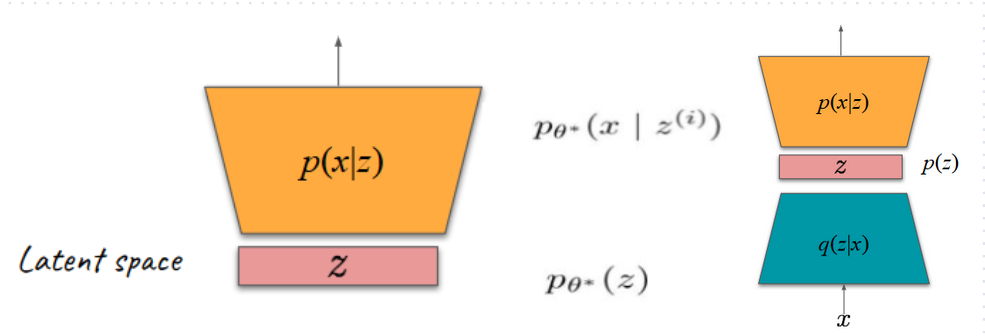
\includegraphics[width=\linewidth]{tikz/VAE posterior.png}
    \caption{{\color{red}\colorbox{pink}{Tikz TO-DO}} The overall image describes the whole flow. In few words, we want to know how to learn how to generate data, x, from our latent variables, z. This implies that we want to learn $p(z|x)$. To learn it, we use the KL distance to approximate the true posterior probability that cannot be computed by bayesian theorem; \textbf{Right}: We can choose prior p(z) to be simple, e.g. Gaussian; Conditional p(x|z) is complex (generates image) and it is represented with Decored neural network; \textbf{Left}: The additonal probabilistic encoder.}
    \label{fig:VAE-posterior}
\end{figure}





\end{comment}


\subsection{VQVAE}

As you might recall, VAEs consist of 3 parts:

   \begin{enumerate}
       \item  An encoder network that parametrizes the posterior q(z|x) over latents
       \item A prior distribution p(z)
       \item A decoder with distribution p(x|z) over input data
   \end{enumerate}
     
    
Typically we assume this prior and posterior to be normally distributed with diagonal variance. The encoder is then used to predict the mean and variances of the posterior.

In the proposed VQVAE work however, the authors use \textbf{discrete latent variables} (instead of a continuous normal distribution). The posterior and prior distributions are categorical, and the samples drawn from these distributions index an \textbf{embedding table}. In other words:

\begin{enumerate}
    \item Encoders model a categorical distribution, from which we sample and get integral values
    \item  These integral values are used to index a dictionary of embeddings
    \item  The indexed values are then passed into the decoder

\end{enumerate}


Many important real-world objects are discrete. For example in images we might have categories like “Cat”, “Car”, etc. and it might not make sense to interpolate between these categories. Discrete representations are also easier to model since each category has a single value whereas if we had a continuous latent space then we will need to normalize this density function and learn the dependencies between the different variables which could be very complex.

\begin{figure}[!htbp]
    \centering
    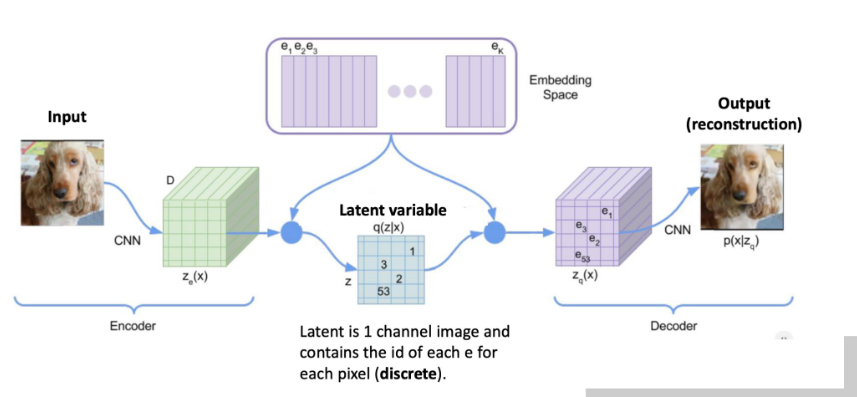
\includegraphics[width=1\linewidth]{tikz/VQVAE.png}
    \caption{{\color{red}\colorbox{pink}{Tikz TO-DO}} VQVAE architecture}
    \label{fig:VQVAE}
\end{figure}

With this new settings (Figure \ref{fig:VQVAE}):

\begin{enumerate}
    \item the Encoder takes in images $x: (n, h, w, c)$ and give outputs $z_e: (n, h, w, d)$, where $d$ are the number of channels in the hidden state.
    \item \textbf{Vector Quantization layer} takes $z_e$ and selects embeddings from a dictionary based on distance and outputs $z_q$.
    \item Decoder consumes $z_q$ and outputs x’ trying to recreate input x
\end{enumerate}

The job done by a VQ layer can be explained in six steps as numbered in Fig \ref{fig:Vector-Quantization-layer}:


\begin{enumerate}
    \item Reshape: all dimensions except the last one are combined into one so that we have n*h*w vectors each of dimensionality d
    \vspace{ 5 pt}
    
    \item Calculating distances: for each of the n*h*w vectors we calculate distance from each of k vectors of the embedding dictionary to obtain a matrix of shape (n*h*w, k)
    \vspace{ 5 pt}
    
    \item Argmin: for each of the n*h*w vectors (for each row) we find the index of closest of the k vectors from dictionary. The latent is 1 channel image $(n*h*w,1)$
    \vspace{ 5 pt}
    
    \item Index from dictionary: index the closest vector from the dictionary for each of n*h*w vectors
    \vspace{ 5 pt}
    
    \item Reshape: convert back to shape (n, h, w, d)
    \vspace{ 5 pt}
    
    \item Copying gradients: If you followed up till now you’d realize that it’s not possible to train this architecture through backpropagation as the gradient won’t flow through argmin. Hence we try to approximate by copying the gradients from $z_q$ back to $z_e$. In this way we’re not actually minimizing the loss function but are still able to pass some information back for training.
\end{enumerate}

\begin{figure}[!htbp]
    \centering
    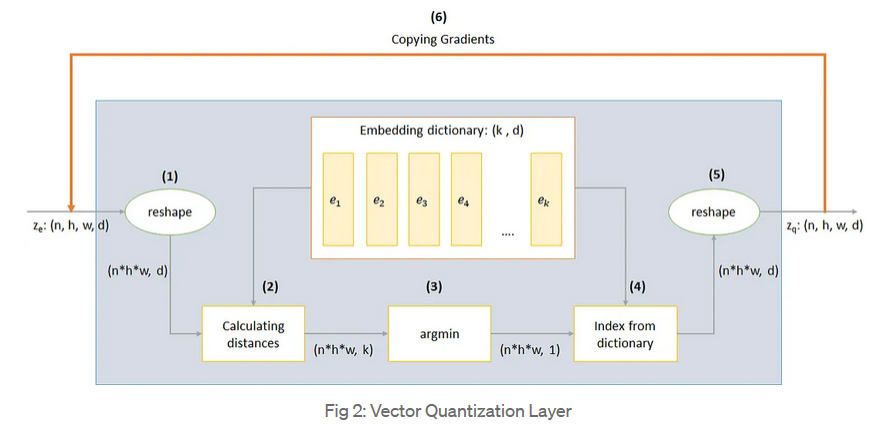
\includegraphics[width=\linewidth]{tikz/VQVAE Vector Quantization .png}
    \caption{{\color{red}\colorbox{pink}{Tikz TO-DO}} A recap of the vactor quantization layer procedure}
    \label{fig:Vector-Quantization-layer}
\end{figure}
    
    
    
    
    
    

\section{GAN vs VAE}

\textbf{GANs} provide a mechanism for generating samples. During training, the GAN loss function encourages these samples to become progressively less distinguishable from real data; \textbf{VAE} are probabilistic models that learn a probability distribution over the
training data. This distribution can be used to draw new samples, and assess the probability of new data points.


\textbf{Comparing GANs and VAEs through Generavite model properties}

\textbf{High-Quality Sampling}: Both GANs and VAEs are capable of high-quality sampling, meaning the samples they generate are often indistinguishable from real data.

\textbf{Coverage}: GANs often struggle with coverage, meaning they might only generate samples that look like a subset of the training data, rather than representing the entire distribution. VAEs generally aim to cover the full distribution, though their success in this area can vary.

\textbf{Well-Behaved Latent Space}: Both models have well-behaved latent spaces. In other words, each latent variable $z$ corresponds to a realistic data example $x$, and smooth changes in $z$ lead to smooth changes in $x$.

\textbf{Interpretable Latent Space}: Neither GANs nor VAEs excel at having an interpretable latent space. Ideally, changing each dimension of $z$ would change a specific, understandable feature of the data, but this is not effectively achieved by either model.

\textbf{Efficient Likelihood Computation}: VAEs struggle with efficiently computing likelihoods, despite being probabilistic models. GANs do not use likelihoods, so this property is not applicable to them.

---
